\documentclass[12pt]{article}
\usepackage[utf8]{inputenc}
\usepackage[T2A]{fontenc}
\usepackage[english,russian]{babel}
\usepackage{amsmath,amssymb}
\usepackage{indentfirst}
\usepackage{hyperref}
\usepackage{graphicx}
\usepackage{placeins}

\hypersetup {
	colorlinks=true
}

\newcommand{\pd}[2]{\frac{\partial #1}{\partial #2}}
\newcommand{\dpd}[2]{\dfrac{\partial #1}{\partial #2}}
\renewcommand{\arraystretch}{1.2}
\let\dividesymbol\div
\renewcommand{\div}{\operatorname{div}}
\newcommand{\grad}{\operatorname{grad}}
\newcommand{\bvec}[1]{\boldsymbol{\mathbf{#1}}}
\newcommand{\cutefrac}[2]{{}^{#1}\mkern-5mu/{\!}_#2}
\newcommand{\half}{{\cutefrac{1}{2}}}
\renewcommand{\iiint}{\int\hspace{-10pt}\int\hspace{-10pt}\int}
\newcommand{\oiint}{%
{}\subset\hspace{-6pt}\supset\hspace{-17.8pt}%
\int\hspace{-10pt}\int%
}%

\author{Цыбулин Иван}
\title{Описание программы \texttt{ellipt}}

\begin{document}
\maketitle

\tableofcontents

\section{Общие сведения}

Программа \texttt{ellipt} предназначена для решения эллиптических уравнений в двумерных областях. Она предлагается в качестве замены существующей программе \texttt{Ellipt2D.exe}, использовавшейся для выполнения третьей лабораторной работы ранее.

Функционально программа \texttt{ellipt} состоит из блока генерации расчетной сетки по описанию области на специальном языке, блока построения разностной схемы с положительной аппроксимацией и расчетного блока. Результат работы программы сохраняется в формате \texttt{VTK}, совместимом с программой визуализации \texttt{Paraview}.

Для работы программе необходимо передать файл с описанием задачи, например в консоли Linux:
\begin{verbatim}
user@host$ ./ellipt64 square.geom
\end{verbatim}
или в консоли (cmd.exe) Windows:
\begin{verbatim}
C:\User> ellipt32.exe square.geom
\end{verbatim}
Программа собрана для Linux и Windows в 32 и 64 битном варианте.

Для описания области используется технология конструктивной геометрии. В качестве базовых доступны всего два примитива --- круг и многоугольник. К любым двум объектам может быть применена одна из следующих операций: пересечение, объединение или вычитание.

На границе каждого объекта необходимо задать граничное условие, даже если эта граница не будет присутствовать результирующей области.

\section{Формат конфигурационного файла}
Конфигурационный файл является простым текстовым файлом на специальном языке программирования. 
Пустые строки и переносы строк игнорируются. В файле допустимы комментарии, начинающиеся с символа \verb|#| и заканчивающиеся в конце строки.
\begin{verbatim}
# Это комментарий

z = (0, 5) # Определяем точку x
\end{verbatim}

Файл состоит из определения произвольного числа переменных, в том числе переменных может не быть вовсе.
Определение переменной состоит из имени переменной слева от знака равенства и значения справа. Каждая переменная может принимать одно из четырех типов значений:
\begin{itemize}
	\item точка;
	\item граничное условие;
	\item область;
	\item уравнение.	
\end{itemize}

После определений переменных должна идти строка
\begin{verbatim}
solve <equation> in <domain> meshsize <hint> [hbnd] [bndAspect]
\end{verbatim}
где вместо \verb|<equation>| должно стоять либо уравнение, либо переменная имеющая тип уравнения. Аналогично, вместо \verb|<domain>| должно стоять определение области либо переменная. Последние три величины \verb|<hint>|, \verb|[hbnd]|, \verb|[bndAspect]| задают размеры сетки. Последние два числа необязательны. Величина \verb|hint| задает характерный шаг внутри области, \verb|hbnd| --- шаг на границе области, \verb|bndAspect| --- расстояние между приграничными слоями точек по отношению к \verb|hbnd|. Если не указывать \verb|bndAspect| будет использовано число $1$, если не указать \verb|hbnd|, он будет выбран равным \verb|hint|.

\subsection{Задание граничных условий}
Для задания граничного условия используется ключевое слово \verb|bndcond|. Далее в фигурных скобках указывается величина, которая должна обнуляться на данной границе. Эта величина может представлять выражение, содержащее координаты точки на границе $x, y$, значение $u$ и значение нормальной производной $\pd{u}{n}$. Пример:
\begin{verbatim}
dirichlet = bndcond { u }
neumann = bndcond { dudn - sin(x) }
robin = bndcond { dudn + 3 * u - x^2 - y^2 }
\end{verbatim}
Здесь заданы три разные переменные --- \verb|dirichlet|, \verb|neumann| и \verb|robin|, представляющие собой условия Дирихле, Неймана и Робина:
\begin{align*}
u\big|_{\partial D} &= 0\\
\pd{u}{n}\Big|_{\partial D} &= \sin x\\
\pd{u}{n} + 3u\Big|_{\partial D} &= x^2 + y^2.
\end{align*}
Поддерживаются только условия, где перед $u, \pd{u}{n}$ стоят постоянные коэффициенты. Свободный член может быть любой функцией $x, y$.

\subsection{Задание областей}
\subsubsection{Задание круга}
Чтобы задать круг используется ключевое слово \verb|circle|. За ним должны следовать координаты центра, радиус и граничное условие.
\begin{verbatim}
# Круг радиуса 5 с центром в точке (0, 0) с условием Дирихле
circ1 = circle (0, 0) radius 5 { u }

z = (3, 5)                      # Точка - центр будущего круга
neumann = { dudn }              # Условия Неймана du/dn = 0

# Круг радиуса 10 с центром в точке z и условиями neumann
circ2 = circle z radius 10 neumann
\end{verbatim}

\subsubsection{Задание многоугольника}
Многоугольник может иметь произвольное число вершин, не меньшее трех. На каждом ребре многоугольника можно задавать свои граничные условия. Обход многоугольника должен происходить против часовой стрелки, иначе его нормали окажутся вывернутыми наизнанку. Начало многоугольника указывается словом \verb|polygon|. Чтобы указать конец списка точек многоугольника используется \verb|close|. Между последовательными вершинами многоугольника должны быть указаны граничные условия на соответствующем ребре. После последней вершины указываются граничные условия на ребре, соединяющем ее с начальной точкой (многоугольник замкнут). Примеры многоугольников
\begin{verbatim}
z1 = (0, 0)
z2 = (1, 0)
z3 = (0, 1)
cond = bndcond { u - x - y }
poly1 = polygon z1 cond z2 cond z3 cond close

poly2 = 
  polygon
    ( 1,  1)
    bndcond { u }
    (-1,  1)
    bndcond { dudn }
    (-1, -1)
    bndcond { u - 1 }
    ( 1, -1)
    bndcond { dudn }
  close
\end{verbatim}

\subsubsection{Операции с областями}
Области можно пересекать операцией \verb|intersect| или \verb|*|, объединять операцией \verb|union| или \verb|+| и вычитать операцией \verb|subtract| или \verb|-|. При необходимости можно брать выражения в скобки. Приоритет вычитания и объединения одинаков и меньше, чем у умножения. Примеры операций с областями
\begin{verbatim}
outer = circle (0, 0) radius 4
          bndcond { u - 4 * sin(5 * atan2(y, x)) }
inner = circle (0, 0) radius 2 bndcond { u }
annulus = outer - inner    # Кольцо - разность двух окружностей

p = polygon
      ( 1,  1) bndcond { u } (-1,  1) bndcond { u }
      (-1, -1) bndcond { u } ( 1, -1) bndcond { dudn }
    close

c = circle (0, 0) radius 1.2 bndcond { dudn + u - 1 }

# Область - пересечение p и c - кривоугольный восьмиугольник
solve elliptic { uxx + uyy } in p * c meshsize 0.05
\end{verbatim}

\subsection{Задание уравнения}
Уравнение задается таким же способом как и граничные условия. Для задания уравнения используется ключевое слово \verb|elliptic|, за которым следует величина, которая должна обращаться в ноль в области. В уравнение могут входить переменные \verb|uxx|, \verb|uxy|, \verb|uyy|, \verb|ux|, \verb|uy|, \verb|u|, а также координаты точки \verb|x|, \verb|y|. Коэффициенты перед производными $u_{xx}, u_{xy}, u_{yy}, u_{x}, u_{y}$ и значением $u$ должны быть постоянными. Свободный член может быть произвольной функцией координат. Пример:
\begin{verbatim}
poisson = { uxx + uyy - x - y }
laplace = { uxx + uyy }
\end{verbatim}
Заданы два уравнения --- Пуассона
$$
\Delta u = x + y
$$
и Лапласа
$$
\Delta u = 0.
$$

\subsection{Задание параметров сетки}
Конфигурация сетки задается тремя параметрами --- $h_\text{int}, h_\text{bnd}$ и $\text{aspect}$.
Внутри области строится равномерная треугольная сетка с шагом $h_\text{int}$, на границах строится сетка с шагом $h_\text{bnd}$. В каждой точке границы в направлении против нормали (внутрь области) добавляется еще три точки с шагом $\text{aspect} \cdot h_\text{bnd}$.

Рекомендуется выбирать $h_\text{bnd} \approx 0.7 h_\text{int}$ и $\text{aspect} = 0.5 \dividesymbol 1$. Программа делает десять итераций по удалению плохих точек. Плохими точками считаются точки, в которых не удается аппроксимировать схему с положительными коэффициентами.
Как только на очередной итерации плохие точки не обнаружены, программа переходит к решению уравнения.

\begin{verbatim}
solve 
  elliptic { uxx + uyy - 1 }
in
  circle (0, 0) radius 1
  bndcond { u }
meshsize 0.1 0.07 0.6
\end{verbatim}
Полученная сетка изображена на рисунке.
\begin{figure}[!ht]
\centering
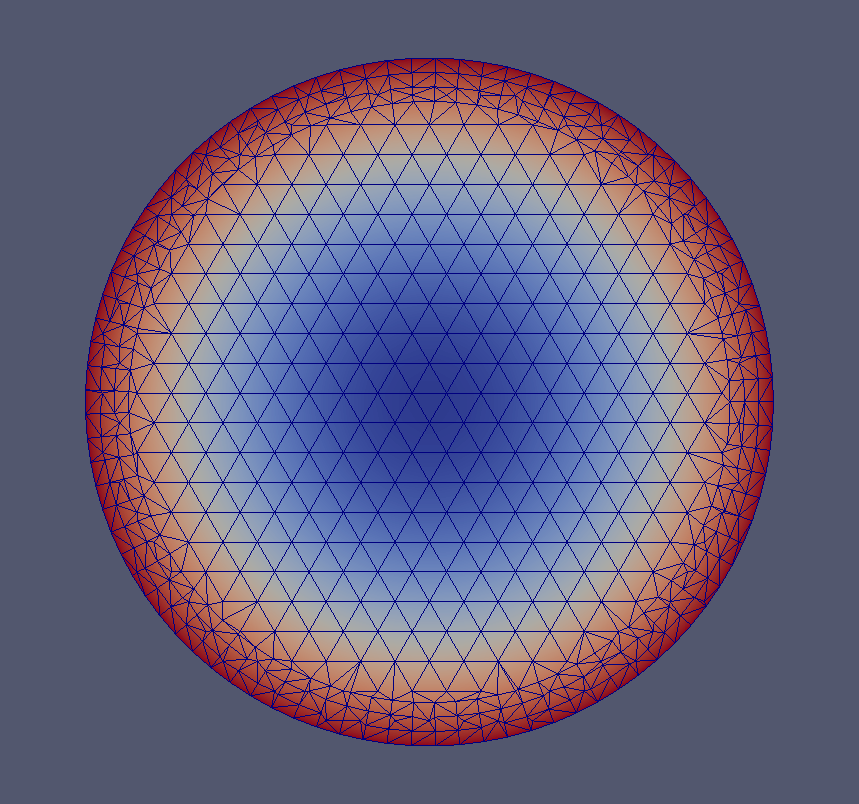
\includegraphics[width=.5\textwidth]{mesh.png}
\end{figure}

\FloatBarrier
\section{Визуализация решения}

Программа делает $10^7$ итераций, сохраняя каждые $10000$ итераций решение в файле формата \texttt{VTK}. Если на итерациях решение меняется в равномерной норме менее чем на $10^{-6}$, процесс останавливается. Сохраняемые файлы имеют названия вида 

\verb|<имя конфигурационного файла>.<номер итерации>.vtk|

Файлы помещаются в ту же директорию, из которой брался конфигурационный файл, то есть
\begin{verbatim}
user@host $ ./ellipt64 ../square.geom
\end{verbatim}
будет сохранять файлы \verb|square.geom.<n>.vtk| на уровень выше, там где находится \verb|square.geom|.

Для просмотра файлов \verb|VTK| используется программа \texttt{Paraview}, которая может быть взята с официального сайта 

\url{http://www.paraview.org/download/}

\end{document}
